\documentclass{beamer}

\title{Brancher AnyBlok à 14 ans d'historique métier}
\subtitle{Une histoire terrifiante de PHP, MySQL et MsSQL}
\author{Jean-Sébastien SUZANNE et Hugo QUEZADA}
\date{2 novembre 2019}

\newcommand{\TwitterLogo}{\protect
\includegraphics[height=
1.7ex,keepaspectratio]{./twitter.png}}
\newcommand{\EmailLogo}{\protect
\includegraphics[height=
1.7ex,keepaspectratio]{./email.png}}
\newcommand{\AnyBlokLogo}{\protect
\includegraphics[height=
1.7ex,keepaspectratio]{./anyblok.png}}

\usepackage{hyperref}
\usepackage{color}

\usetheme{Amsterdam}
\begin{document}
	\frame {
		\titlepage
	}
	
	\frame {
		\frametitle{Qui sommes nous ?}
		
		\begin{columns}
            \begin{column}{3cm}
                \begin{figure}
  					
\includegraphics[width=\linewidth]{logosensee-carre.jpg}
  					\label{fig:sensee}
				\end{figure}
			\end{column}
			\begin{column}{3cm}
				\begin{figure}
  					
\includegraphics[width=\linewidth]{lentillesmoinscheres-mobile.png}
  					\label{fig:lmc}
				\end{figure}
			\end{column}
		\end{columns} 			
		\begin{columns}
            \begin{column}{5cm}
                \textbf{\AnyBlokLogo{} Sébastien Suzanne}
		    	\begin{itemize}
			  		\item Répond aussi au nom de PAPABLOK
			  		\item \TwitterLogo{} @jssuzanne
			    	\item \EmailLogo{} js.suzanne@sensee.com
		    	\end{itemize}
			\end{column}
			\begin{column}{5cm}
				\textbf{Hugo Quezada}
		    	\begin{itemize}
			  		\item Dis le petit Basque du Chili
			  		\break
			    	\item \EmailLogo{} h.quezada@sensee.com
		    	\end{itemize}
			\end{column}
		\end{columns}
	}
	
	\frame{
		\frametitle{Existant}
		\framesubtitle{14 ans de code...}
		\begin{itemize}
			\pause
			\item Code legacy en PHP5 (pas de troll SVP)
			\item Pas de framework, beaucoup de code, très peu d'objet
			\break
			\pause
			\item Pas de tests
			\item Pas de CI
			\break
			\pause
			\item Pas d'ORM
		\end{itemize}
	}
	
	\frame{
		\frametitle{Existant}
		\framesubtitle{Une BdD un peu complexe...}
		\begin{itemize}
			\item  Schémas de base de données multiples
			\pause
			\item  Écosystème avec plusieurs SGBD (MySQL, MsSQL) souvent sans API
			\begin{figure}[p]
				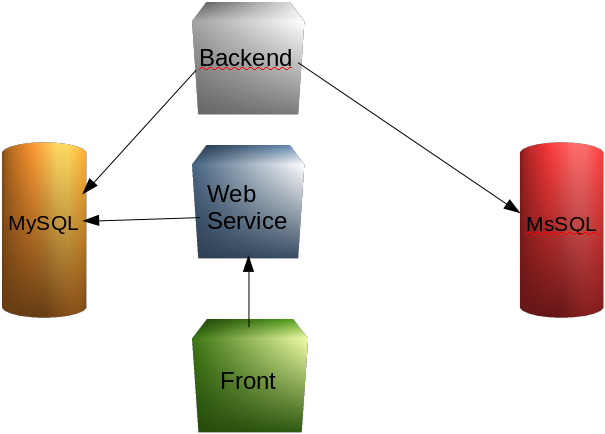
\includegraphics[height=25ex,keepaspectratio]{./schema_simplifie_lmc.png}
				\caption{Schéma simplifié}
			\end{figure}
		\end{itemize}
	}
	
	\frame{
		\frametitle{Vision finale}
		\framesubtitle{L'objectif}
		\begin{itemize}
		    \item Un code python propre et testé
			\item Une API simple et uniforme, utilisé dans tous nos projets
			\item Une application plus proche des standards actuels
			\item Un projet plus séduisant et plus attrayant pour des potentiels futurs développeurs 
		\end{itemize}
	}
	\frame{
		\frametitle{Vision finale}
		\framesubtitle{La stratégie}
		\begin{itemize}
			\item Modèle d'étranglement (Strangle pattern)
			\begin{figure}[p]
				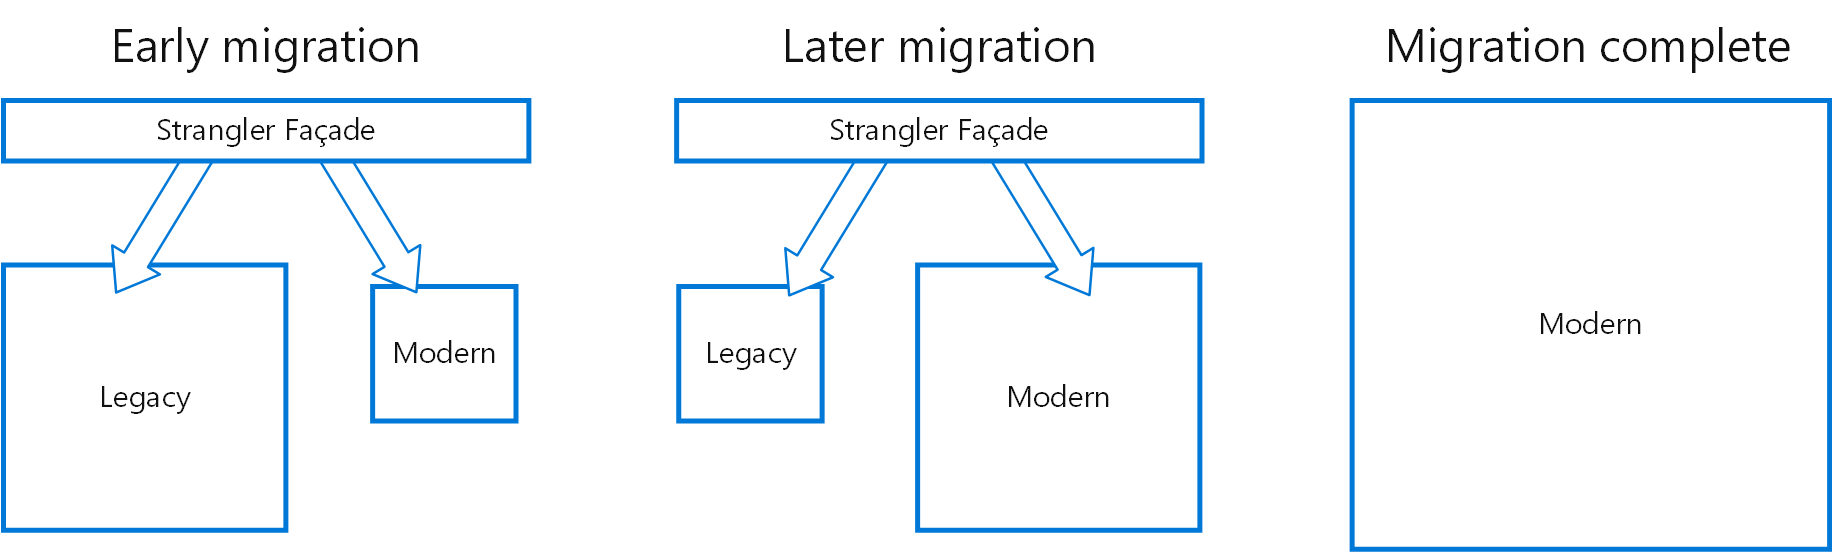
\includegraphics[height=15ex,keepaspectratio]{./strangler.png}
			\end{figure}
			\item Mapping des tables avec un nommage plus clair
			\item Développement piloté par les tests (TDD)
		\end{itemize}
	}
	\frame{
		\frametitle{Pourquoi avoir choisi AnyBlok ?}
		\framesubtitle{AnyBlok: Présentation}
	}
	\frame{
		\frametitle{Pourquoi avoir choisi AnyBlok ?}
		\framesubtitle{AnyBlok: Écrire des tests pour notre Model}
	}
	\frame{
		\frametitle{Pourquoi avoir choisi AnyBlok ?}
		\framesubtitle{AnyBlok: Définir le Model}
	}
	\frame{
		\frametitle{Pourquoi avoir choisi AnyBlok ?}
		\framesubtitle{AnyBlok: Définir un Model sur une table existante}
	}
	\frame{
		\frametitle{Pourquoi avoir choisi AnyBlok ?}
		\framesubtitle{AnyBlok: Créer API web et tests unitaires associés}
	}
	\frame{
		\frametitle{Pourquoi avoir choisi AnyBlok ?}
		\framesubtitle{AnyBlok: Créer un console script dédié par service}
	}
	\frame{
		\frametitle{Evolutions et intégrations dans AnyBlok}
		\framesubtitle{Compatibilité avec MySQL}
		
		\pause
		\begin{itemize}
			\item 2 semaines de travails
			\item beaucoup de recherche et d'incompréhension 
		\end{itemize}
	}	
	\frame{
		\frametitle{Evolutions et intégrations dans AnyBlok}
		\framesubtitle{Compatibilité avec MySQL: Les tests unitaires}
		
		\begin{itemize}
			\item Mise a jour de configuration travis-ci
			\item \pause Activer le mode transactionnel de innoDB
			\item \pause {\color{blue}\href{https://dev.mysql.com/doc/refman/8.0/en/implicit-commit.html}{Les commits implicites}}
		\end{itemize}
	}	
	\frame{
		\frametitle{Evolutions et intégrations dans AnyBlok}
		\framesubtitle{Compatibilité avec MySQL: Limitation}
		
		\begin{itemize}
			\item Pas de Python 3.5
			\item \pause Pas de CheckConstrainte et autre containte exclusive a PostgrSQL
			\item \pause Datetime naives
			\item \pause Pas de chiffrement sur les columns UUID
			\item \pause Pas de véritable Boolean
		\end{itemize}
	}	
	\frame{
		\frametitle{Evolutions et intégrations dans AnyBlok}
		\framesubtitle{Compatibilité avec MariaDB}
		
		\begin{itemize}
			\item Pas de Python 3.5
			\item Pas de CheckConstrainte et autre containte exclusive a PostgrSQL
			\item Datetime naives
			\item Pas de chiffrement sur les columns UUID
			\item Pas de véritable Boolean
			\item \pause taille des clé primaires plus petite
			\item \pause Pas de colonnes JSON
		\end{itemize}
	}
	\frame{
		\frametitle{Evolutions et intégrations dans AnyBlok}
		\framesubtitle{Compatibilité avec MsSQL}
		
		\begin{itemize}
			\item Pas de Python 3.5
			\item Pas de CheckConstrainte et autre containte exclusive a PostgrSQL
			\item \pause lent
		\end{itemize}
	}
	\frame{
		\frametitle{Evolutions et intégrations dans AnyBlok}
		\framesubtitle{Définition de schémas}
		Choix
		\begin{itemize}
			\item c'est dans la reprise de donnée
			\item Programmatique ou Configuration
			\item Poser sur un modèle ou un namespace
			\item Ajout de suffixes ou préfixes pour les tests
		\end{itemize}
		\hfill \linebreak
		Problématiques
		\begin{itemize}
			\item génération de foreign key
			\item migration
		\end{itemize}
	}
	\frame{
	exemple programatique
	exemple configuration
	}
	\frame{
		\frametitle{Fin}
		\begin{columns}
			\begin{column}{4cm}
			\end{column}
			\begin{column}{8cm}
				Des questions ? 
				\break
				Des remarques ?
			\end{column}
		\end{columns}
	}
		
\end{document}
